%%
%% This is file `sample-sigconf.tex',
%% generated with the docstrip utility.
%%
%% The original source files were:
%%
%% samples.dtx  (with options: `all,proceedings,bibtex,sigconf')
%% 
%% IMPORTANT NOTICE:
%% 
%% For the copyright see the source file.
%% 
%% Any modified versions of this file must be renamed
%% with new filenames distinct from sample-sigconf.tex.
%% 
%% For distribution of the original source see the terms
%% for copying and modification in the file samples.dtx.
%% 
%% This generated file may be distributed as long as the
%% original source files, as listed above, are part of the
%% same distribution. (The sources need not necessarily be
%% in the same archive or directory.)
%%
%%
%% Commands for TeXCount
%TC:macro \cite [option:text,text]
%TC:macro \citep [option:text,text]
%TC:macro \citet [option:text,text]
%TC:envir table 0 1
%TC:envir table* 0 1
%TC:envir tabular [ignore] word
%TC:envir displaymath 0 word
%TC:envir math 0 word
%TC:envir comment 0 0
%%
%%
%% The first command in your LaTeX source must be the \documentclass
%% command.
%%
%% For submission and review of your manuscript please change the
%% command to \documentclass[manuscript, screen, review]{acmart}.
%%
%% When submitting camera ready or to TAPS, please change the command
%% to \documentclass[sigconf]{acmart} or whichever template is required
%% for your publication.
%%
%%
\documentclass[sigconf]{acmart}

\usepackage{subcaption}

%%
%% \BibTeX command to typeset BibTeX logo in the docs
\AtBeginDocument{%
  \providecommand\BibTeX{{%
    Bib\TeX}}}

%% Rights management information.  This information is sent to you
%% when you complete the rights form.  These commands have SAMPLE
%% values in them; it is your responsibility as an author to replace
%% the commands and values with those provided to you when you
%% complete the rights form.
\setcopyright{acmlicensed}
\copyrightyear{2018}
\acmYear{2018}
\acmDOI{XXXXXXX.XXXXXXX}

%% These commands are for a PROCEEDINGS abstract or paper.
\acmConference[Conference acronym 'XX]{Make sure to enter the correct
  conference title from your rights confirmation emai}{June 03--05,
  2018}{Woodstock, NY}
%%
%%  Uncomment \acmBooktitle if the title of the proceedings is different
%%  from ``Proceedings of ...''!
%%
%%\acmBooktitle{Woodstock '18: ACM Symposium on Neural Gaze Detection,
%%  June 03--05, 2018, Woodstock, NY}
\acmISBN{978-1-4503-XXXX-X/18/06}


%%
%% Submission ID.
%% Use this when submitting an article to a sponsored event. You'll
%% receive a unique submission ID from the organizers
%% of the event, and this ID should be used as the parameter to this command.
%%\acmSubmissionID{123-A56-BU3}

%%
%% For managing citations, it is recommended to use bibliography
%% files in BibTeX format.
%%
%% You can then either use BibTeX with the ACM-Reference-Format style,
%% or BibLaTeX with the acmnumeric or acmauthoryear sytles, that include
%% support for advanced citation of software artefact from the
%% biblatex-software package, also separately available on CTAN.
%%
%% Look at the sample-*-biblatex.tex files for templates showcasing
%% the biblatex styles.
%%

%%
%% The majority of ACM publications use numbered citations and
%% references.  The command \citestyle{authoryear} switches to the
%% "author year" style.
%%
%% If you are preparing content for an event
%% sponsored by ACM SIGGRAPH, you must use the "author year" style of
%% citations and references.
%% Uncommenting
%% the next command will enable that style.
%%\citestyle{acmauthoryear}


%%
%% end of the preamble, start of the body of the document source.
\begin{document}

%% 
%% The "title" command has an optional parameter,
%% allowing the author to define a "short title" to be used in page headers.
\title{Spreadsheet Data Extractor}

%%
%% The "author" command and its associated commands are used to define
%% the authors and their affiliations.
%% Of note is the shared affiliation of the first two authors, and the
%% "authornote" and "authornotemark" commands
%% used to denote shared contribution to the research.
\author{Alexander Aue-Johr}
%\authornote{Both authors contributed equally to this research.}
\email{alexander.aue@thuenen.de}
\orcid{0009-0001-8683-3630}
\affiliation{%
  \institution{Institute of Rural Studies of the Johann Heinrich von Thünen-Institute}
  \city{Brunswick}
  \country{Germany}
}


 
%%
%% By default, the full list of authors will be used in the page
%% headers. Often, this list is too long, and will overlap
%% other information printed in the page headers. This command allows
%% the author to define a more concise list
%% of authors' names for this purpose.
\renewcommand{\shortauthors}{Trovato et al.}

%%
%% The abstract is a short summary of the work to be presented in the
%% article.
\begin{abstract}
  Spreadsheet data often exists in a semi-structured format that presents challenges for data analysis and processing. The Spreadsheet Data Extractor (SDE) addresses these issues by offering a user-centric interface to transform Excel data into structured formats. Significant improvements in performance have been achieved by custom parsing of Excel files and incremental loading of sheets, leading to faster operations on large workbooks compared to conventional methods. Rendering efficiency has also been optimized by calculating cell positions dynamically based on viewport scrolling, ensuring only visible cells are processed, which drastically improves usability for large spreadsheets.
  \end{abstract}

%%
%% The code below is generated by the tool at http://dl.acm.org/ccs.cfm.
%% Please copy and paste the code instead of the example below.
%%
\begin{CCSXML}
<ccs2012>
 <concept>
  <concept_id>00000000.0000000.0000000</concept_id>
  <concept_desc>Do Not Use This Code, Generate the Correct Terms for Your Paper</concept_desc>
  <concept_significance>500</concept_significance>
 </concept>
 <concept>
  <concept_id>00000000.00000000.00000000</concept_id>
  <concept_desc>Do Not Use This Code, Generate the Correct Terms for Your Paper</concept_desc>
  <concept_significance>300</concept_significance>
 </concept>
 <concept>
  <concept_id>00000000.00000000.00000000</concept_id>
  <concept_desc>Do Not Use This Code, Generate the Correct Terms for Your Paper</concept_desc>
  <concept_significance>100</concept_significance>
 </concept>
 <concept>
  <concept_id>00000000.00000000.00000000</concept_id>
  <concept_desc>Do Not Use This Code, Generate the Correct Terms for Your Paper</concept_desc>
  <concept_significance>100</concept_significance>
 </concept>
</ccs2012>
\end{CCSXML}

\ccsdesc[500]{Do Not Use This Code~Generate the Correct Terms for Your Paper}
\ccsdesc[300]{Do Not Use This Code~Generate the Correct Terms for Your Paper}
\ccsdesc{Do Not Use This Code~Generate the Correct Terms for Your Paper}
\ccsdesc[100]{Do Not Use This Code~Generate the Correct Terms for Your Paper}

%%
%% Keywords. The author(s) should pick words that accurately describe
%% the work being presented. Separate the keywords with commas.
\keywords{Do, Not, Us, This, Code, Put, the, Correct, Terms, for,
  Your, Paper}
%% A "teaser" image appears between the author and affiliation
%% information and the body of the document, and typically spans the
%% page.
\begin{teaserfigure}
  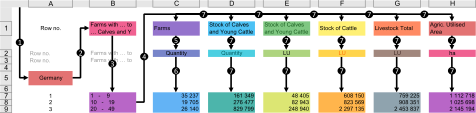
\includegraphics[width=\textwidth]{images/spreadsheet_data_extractor/livestock_hiarachy_1.pdf}
  \caption{Seattle Mariners at Spring Training, 2010.}
  \Description{Enjoying the baseball game from the third-base
  seats. Ichiro Suzuki preparing to bat.}
  \label{fig:teaser}
\end{teaserfigure}

\received{20 February 2007}
\received[revised]{12 March 2009}
\received[accepted]{5 June 2009}

%%
%% This command processes the author and affiliation and title
%% information and builds the first part of the formatted document.
\maketitle


\section{Introduction}
\cite{R}
A multitude of organizations across various sectors,
including healthcare\cite{berndt2001healthcare},
nonprofit\cite{singh2009numeric}\textsuperscript{,}
\cite{west2008because},
finance, commerce, industry, academia, and government \cite{dunn2010spreadsheets}
use semi-structured data stored in spreadsheets, which presents challenges for analysis due to the lack of a predefined structure.

With our Spreadsheet Data Extractor we build upon previous developments by Alexander Aue, Norbert Röder, and Andrea Ackermann, who developed a tool for extracting data from spreadsheets \cite{alexander2024converting}. However, their implementation relied on external libraries, which negatively impacted the program's performance. Our current version introduces a custom Excel parser and an incremental sheet-loading mechanism, making it faster and more efficient than Excel itself in handling large workbooks. To further optimize performance, we improved the rendering efficiency by dynamically calculating cell positions based on viewport scrolling. This ensures that only visible cells are processed, significantly enhancing usability when interacting with large tables. The Thünen Institute granted us permission to release the improved the GPL v3 license. We also conceptualized 
  


\begin{figure*}[t]
  \centering

  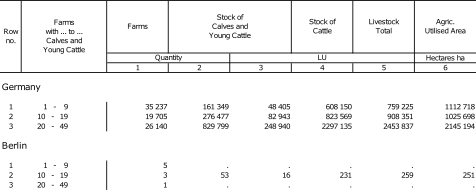
\includegraphics[width=\textwidth]{images/spreadsheet_data_extractor/livestock.pdf}

  \caption[Example data subset of the Agricultural Structure Survey on land use and livestock in Germany]{Example data subset of the Agricultural Structure Survey on land use and livestock in Germany, Source: Own figure}
  
  \label{fig:livestock}
\end{figure*}%

Nevertheless, it is not always the case that there is no structure at all.
There are cases where the data at least has "a" structure.
However, this structure is almost as helpful
as if there were simply none at all.
This is the case for data stored in spreadsheet files like Excel.
The data is not stored in a simple machine-readable wide- or long-format;
rather, it is stored in a format that is designed for human perception,
including layout with empty cells for padding, combined cells,
hierarchies in column headers, multiple tables below one another, and so on.
This is illustrated in Figure \ref{fig:livestock}
These layout techniques facilitate the comprehension of the information
by humans, but they also render the data non-machine readable.
A computer program treats the spreadsheet
as a two-dimensional array of values.
It treats empty cells in the same way
as it treats cells that contain actual data.



 


Compared to unstructured data in raw text, unstructured data in spreadsheets has the following advantages:
The hierarchy of metadata within spreadsheets is easy to comprehend for a human.
Headlines like \textit{Germany} and \textit{Berlin},
referring to our example in Figure \ref{fig:livestock},
combined column headers like \textit{Stock of Calves and Young Cattle}
on top of multiple other column headers like \textit{Quantity} and \textit{LU}
make the metadata hierarchy clear to humans.
The target data structure can be closely inspired by that visible hierarchy
and can be created with a relatively low amount of domain knowledge.
Furthermore, the values are encoded in single cells and can be uniquely
referenced by the file, sheet name and row and column index. 

In contrast, the target data structure for raw text documents is not as explicit as in spreadsheets.
Rather, it is implicit and must be created from scratch,
requiring a significant amount of domain knowledge.
Furthermore, data in prose text documents is represented in sentences, requiring human interpretation.

However, the fundamental problem of both data sources is the same:
there is data with no machine-readable structure.
The objective is to transform this data into a machine-readable form.
When considering the means to achieve this objective,
several approaches present themselves.

One potential avenue is the use of Artificial Intelligence (AI)
to automatically structure the data.
However, it is important to note that although AI recognition approaches achieve a high degree of accuracy,
they rarely reach 100\%.
This is not only true for image analysis but also for text recognition.
The current literature on AI approaches used to recognize data and metadata
indicates an accuracy of around 80\% or 90\%.\cite{dong2019tablesense} 
For image analysis, such a high level of accuracy may be acceptable.
To illustrate, provided that a robot is capable of distinguishing between a plant and a weed with a 90\% success rate, it can apply a herbicide locally to the plant in question, while the remaining 10\% of the weed that is not recognized is likely to be identified in the future when the weed grows out more distinguishable characteristics.

However, if the metadata hierarchy and the data from spreadsheets
or text documents processed by AI are only 90\% accurately recognized,
then it is necessary to check all the data in order to identify
which data was incorrectly recognized. This would be a considerable workload. 

An alternative approach would be to employ a sufficient number of data scientists
who are responsible for structuring and cleansing data from spreadsheets,
as well as application developers and database experts who are tasked
with developing data collection forms and corresponding structured databases
for the purpose of collecting data from text documents.
However, this approach is not a viable solution,
as there are significantly more unstructured data sources than there are data scientists,
developers and database administrators. 



Nevertheless,
there are already numerous individuals with the requisite knowledge in the domain.
One potential solution is to empower these experts to structure the data themselves,
without requiring a steep learning curve. Rather than mastering a programming language,
they could utilize user-friendly graphical user interfaces.
Such tools would enable them to describe the structure of spreadsheets for data extraction
and define the structure of data collection forms and their corresponding database. 

Exactly this is contribution of this dissertation.
As depicted in Figure \ref{fig:venn_diagramms}, we introduce two graphical user interface tools,
to help users convert unstructured data and semi-structured data to structured data:
The Spreadsheet Data Extractor (SDE) and Form Generator (FG).


 

The SDE converts semi-structured spreadsheet data into structured formats
by allowing users to define data hierarchies without programming knowledge.

 


The Spreadsheet Data Extractor (SDE) enables users to transform the data from spreadsheets
into structured data by selecting cells containing metadata
and values to describe the data hierarchy.
To streamline the process,
users can copy previously described hierarchies to similar spaces in the sheets,
eliminating the need to select every cell and hierarchy repeatedly.  
Users do not require any programming knowledge to extract the data from the spreadsheet files.
 
 

\begin{table*}[h]
  \centering
  \begin{tabular}{|c|c|c|c|c|}
      \hline
      \textbf{Name} & \textbf{Technologies} & \textbf{Output} & \textbf{Accessibility} & \textbf{Frequency} \\ \hline
      FlashRelate   & AI, GUI               & cleaned data    & proprietary,           & last publication   \\
                    &                       &                 & no access              & 2015               \\ \hline


      Senbazuru     & AI, GUI               & cleaned data    & open source            & last commit        \\
                    &                       &                 &                        & 2015               \\\hline

      XLindy        & AI                    & cleaned data    & no access              & cancelled          \\ \hline
      TableSense    & AI                    & diagrams        & proprietary,           & last commit        \\
                    &                       &                 & no access              & 2021               \\ \hline
  \end{tabular}
  \caption{Spreadsheet Data Extractor counterparts}

  \label{tab:approaches}
\end{table*}


\section{Related Work}

This chapter will first describe
the similar approaches of data extraction
from spreadsheets without programming 
that are found in scientific literature.

Second similar form generators will be described
and which missing features led to the decision
to  develop n individual form generator.

 

\section{Spreadsheet Data Extractor}




Our program's closest research counterparts
are the projects, Senbazuru,  and FlashRelate,
both of which share the goal of extracting relational data from spreadsheets with a graphical user Interface.
\cite{chen2013senbazuru},\cite{barowy2015flashrelate},\cite{koci2019xlindy} 



Senbazuru aims to automatically infer the hierarchical structure
within spreadsheets through the creation of a classifier
that identifies data frames in the document,
along with another classifier that infers the intended hierarchy
using a predefined set of features \cite{chen2013senbazuru}.

While Senbazuru offers automated inference of the hierarchical structure,
it may occasionally produce errors.
In such cases, the tool allows the user to rectify these errors
in the hierarchy by manually dragging and dropping nodes to their correct parent locations.
Unlike Senbazuru, our program does not automatically infer the hierarchical structure.
Instead, our program lets the user decide if the next selection is a child or a sibling of another selection.
To speed up the process,
selections can be duplicated and moved both horizontally and vertically.
Thus, a hierarchy representing a column can be duplicated and shifted over another column,
and similarly,
a hierarchy representing a table can be duplicated and shifted over another table.



FlashRelate utilizes both positive and negative output examples
to generate a program in a domain-specific language called Flare.\cite{barowy2015flashrelate}  
This approach enables FlashRelate
to handle various extraction tasks
from diverse spreadsheets,
as long as it is possible
to identify cells using regular expressions
and recognize the spatial arrangement of the cells.
In contrast to FlashRelate,
our program necessitates the user
to manually choose each data cell containing
either data or metadata.
It does not automatically identify similar cells
based on user-provided selections.
Instead, our program allows users to select not only individual cells
but also sets of cells.
Portions of the spreadsheet
that represent relational data
rather than hierarchical data
can be chosen by first selecting
the domain of the relation as a set of cells.
Typically, the range values of the relation share the same row as the domain values.
In a subsequent step,
the ranges of the relation can be selected
by duplicating the cell set of the domain
and moving it horizontally to the desired cells containing the range values.

There are also two projects that rely on Artificial Intelligence only to identify the hierarchy of the data inside spreadsheets.
Those projects are XLindy and TableSense.
\cite{koci2019xlindy},\cite{dong2019tablesense}

XLindy is not in development any more.
Attempts were made to contact the authors to try the tool and find out if
using it on our test dataset results in reliable output.
Due to the fact that the project is no longer in development
the  tool could not be obtained and tested.

TableSense employs Convolutional Neural Networks
to identify tables in spreadsheets.\cite{dong2019tablesense}  
In their test with the WebSheet400 dataset,
out of 400 random spreadsheets containing 795 tables,
TableSense successfully detected 91.3\% of the tables (recall),
and of the tables detected by TableSense, 86.5\%
were indeed genuine tables (precision).
However, while TableSense excels at detecting table boundaries,
it does not identify data hierarchy or extract data from the tables it identifies.
Our approach currently does not rely on Artificial Intelligence.
Our project's primary focus is to empower users
to manually select all the desired data and describe its hierarchy,
enabling our program to automatically extract this data into a relational format.


\section{Methodology}

\begin{figure*}[h]
  \begin{subfigure}{1.0\textwidth}
    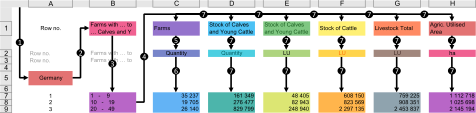
\includegraphics[width=\textwidth]{images/spreadsheet_data_extractor/livestock_hiarachy_1.pdf}
    \caption{The data selection view, once all selections are completed}
    \label{fig:livestock_hiarachy_1}
  \end{subfigure}
  \begin{subfigure}{1.0\textwidth}
    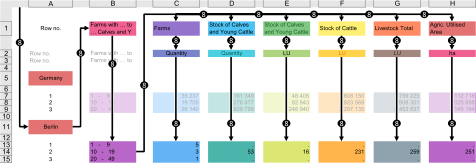
\includegraphics[width=\textwidth]{images/spreadsheet_data_extractor/livestock_hiarachy_2.pdf}
    \caption{The data selection view, once all selections are completed}
    \label{fig:livestock_hiarachy_2}
  \end{subfigure}
  \caption[Second Level Third Level Questions]{Second Level Third Level Questions, Source: Own figure}
  \label{fig:livestock_hiarachy}  
\end{figure*}

We used the software development kit Flutter
to develop a program with a user interface
that allows the selection of the cells containing the metadata
and data inside the spreadsheet.
We refer again to the example from Figure \ref{fig:livestock}
to describe the necessary steps
required for data extraction from spreadsheets.
We use this example spreadsheet to illustrate
the necessary steps required for data extraction
from spreadsheets like this one.
When looking at the spreadsheet,
a human can identify a hierarchy very easily.
There are sub-tables with headings,
and all the sub-tables share the same columns,
which are only laid out once at the top of the spreadsheet
rather than being repeated for each sub-table.

The headings \textit{Germany} and \textit{Berlin} in this example
are the topmost metadata because most cells containing actual data
share these headings as common metadata,
whereas the metadata of the column header \textit{Agric. Utilised Area}
and \textit{Hectares ha} is only shared by the cells beneath that column.
A human can see these hierarchies,
but to a program, these hierarchies are not visible;
the program just sees a two-dimensional grid of cells,
some empty, some containing text, and some containing numbers.

The computer needs to be able to interpret this hierarchy in the spreadsheet
just as a human does.
However, for that to happen, it needs the hierarchy as input.
Our approach is that the user provides this hierarchy
to the computer by selecting the cells and describing the relationships
they have to one another.

To make this process easier and faster for the user,
the amount of user interaction should be minimized as much as possible.
This can be achieved by selecting the most abstract meta-information first
and then progressively narrowing down to increasingly specific meta-information
until the actual facts are chosen.
Additionally, allowing the user to duplicate selections and hierarchies
to similar areas in the spreadsheet can streamline this process.






%\begin{figure*}[!t]
%  \centering
%  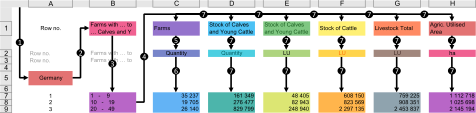
\includegraphics[width=\textwidth]{images/spreadsheet_data_extractor/livestock_hiarachy_1.pdf}
%  \caption{The data selection view, once all selections are completed}
%  \label{fig:livestock_hiarachy_1}
%\end{figure*}




 
In Figure \ref{fig:livestock_hiarachy_1}, cells are presented
as they appear within our program's data selection view
after all the selections are made.
Additionally, an additional layer with black arrows illustrates
the optimal sequence of selections for this example,
designed to minimize user interaction.
These arrows, numbered from 1 to 7, represent the specific steps of user interaction.








Please note that the program deconstructs merged cells.
Cells from which the merged cell was created are displayed as individual cells (e.g. \textit{Quantity} and \textit{LU}).
This will be useful for the following selections.


\begin{figure}[h]
    \centering
 
    \includegraphics[width=0.5\textwidth]{images/spreadsheet_data_extractor/duplicate_and_move.png}
 
    \caption[Selecting the tables arranged one below the other]{Selecting the tables arranged one below the other}
    
    \label{fig:duplicate_and_move}
\end{figure}%

The most abstract meta-information, which is the meta-information shared by most cells, is the country or state in this example (Arrow 1). After that, the header of the domain of the relation is selected (Arrow 2) and then the domain itself will be picked (Arrow 3). While Selections 1 and 2 each selected individual cells, Selection 3 introduces the concept of choosing a set of cells.
Moving on to the first data column, the process involves selecting the first column header (Arrow 4), followed by choosing the second column header (Arrow 5). Now, the first range of the relation is selected (Arrow 6).
If the selection of data were to continue in the same manner, this would involve an additional 15 selections just for the first table, offering no significant improvement over manually creating the relation by simply copying and pasting the cells. However, the subsequent selections can be automated,
given that both two column headers and the numeric values are located in the same row, each one cell to the right of the previous one. The program's \textit{Duplicate and Move} function allows these cells to be selected in a single step.
To do this, Selection 4 is chosen, and the duplicate is moved one cell to the right.

A slider can be adjusted to determine the number of duplicates to generate. Each duplicate is moved the same number of cells in the same direction as the previous one.
For this example, the slider is set to create 5 duplicates (see Figure \ref{fig:duplicate_and_move}).
This results in all the selections depicted as arrows labelled 7 in Figure \ref{fig:livestock_hiarachy_1}.

This functionality is made possible by the Spreadsheet Data Extractor's ability
to deconstruct merged cells, such as those in the \textit{Quantity} and \textit{LU} columns.
Without this feature, duplicating and moving selections over these merged columns would fail,
resulting in the cells within the \textit{Quantity} and \textit{LU} columns remaining empty, except for the first cell in each merged group.
However, the Spreadsheet Data Extractor displays the underlying cells of the merged cells as redundant copies.
This approach allows the process of duplicating and moving column selections over these merged areas to work seamlessly.
With this, the first table is captured.



The same procedure used to capture the previous five columns
can be applied to capture the tables arranged below one another.
To do this, Selection 1 is chosen, then duplicated and moved down by six cells.
However, the header cells (B1 to H2) are an exception to this,
because they don't reappear in the tables below.
The program offers a freeze option for this purpose.
The frozen cells are duplicated but remain in their original positions during the move.
Figure \ref{fig:livestock_hiarachy_2} illustrates how the \textit{Duplicate and Move} function was employed
to capture the table below by moving all but the frozen cells down
by six cells (all arrows labelled with the number 8).


After the selections are made,
the hierarchy of selections forms a tree
in which each node contains the selected set of cells.
Except for the first two nodes,
where the first node represents the spreadsheet file (e.g. \textit{Livestock.xlsx})
and the second node represents the workbook's worksheet (e.g. \textit{Calves}). 
This is demonstrated in Figure \ref{fig:tree_horizontal_small}
for the subtree with the root node \textit{Germany}.


\begin{figure*}[ht]
  \begin{subfigure}{1.0\textwidth}
    \includegraphics[width=\textwidth]{images/spreadsheet_data_extractor/tree_horizontal_small_v2.pdf}
    \caption[Tree structure of cell sets of subtree Germany]{Tree structure of cell sets of subtree Germany, Source: Own figure}
    \label{fig:tree_horizontal_small}
  \end{subfigure}
  \begin{subfigure}{1.0\textwidth}
    \includegraphics[width=\textwidth]{images/spreadsheet_data_extractor/tree_product_horizontal_small_v2.pdf}
    \caption[Cross Product of subtree Germany]{Cross Product of subtree Germany, Source: Own figure}
    \label{fig:tree_product_horizontal_small}
  \end{subfigure}
  \caption[Second Level Third Level Questions]{Second Level Third Level Questions, Source: Own figure}
  \label{fig:livestock_hiarachy}  
\end{figure*}



%%\begin{figure*}[t]
%    \centering
%    \includegraphics[width=\textwidth]{images/spreadsheet_data_extractor/tree_horizontal_small_v2.pdf}
%    \caption[Tree structure of cell sets of subtree Germany]{Tree structure of cell sets of subtree Germany, Source: Own figure}
%    \label{fig:tree_horizontal_small}
%\end{figure*}%


%\begin{figure*}[t]
%  \centering
%  \includegraphics[width=\textwidth]{images/spreadsheet_data_extractor/tree_product_horizontal_small_v2.pdf}
%  \caption[Cross Product of subtree Germany]{Cross Product of subtree Germany, Source: Own figure}
%  \label{fig:tree_product_horizontal_small}
%\end{figure*}%


To transform this tree of sets of cells into relational data,
we calculate the cross product of the tree.
The length of each child set is obtained from the bottom up,
and the parent node is duplicated as many times as necessary
to match the length of that child set (Figure \ref{fig:tree_product_horizontal_small}). 


If the length of the parent and child nodes differ
and the length of the parent set is not a whole number divisor
of the length of the child set,
an error will be thrown,
as it is not possible to duplicate the parent set
to match the length of the child set.
This situation should not occur.
When a parent set consists of more than one cell,
it is usually because the parent set
represents the identifier of the rows,
or in mathematical terms,
the domain of the relation.
This domain must be of the same length as the values represented
to the right of the rows' identifier,
which correspond to the relation range in mathematical terms.
This is also applicable to the table in Figure \ref{fig:livestock},
where the relation's domain comprises
the cells \textit{1-9}, \textit{10-19}, and \textit{20-49},
while the range is located to the right of it.





The final step is to convert each list of sets to tuples
and stack them on top of each other to create the final relation,
as shown in \ref{fig:spreadsheet_data_extractor_output}.
This relation can then be exported as a CSV file.


\begin{figure*}[t]
    \centering
    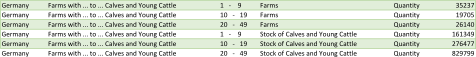
\includegraphics[width=0.5\textwidth]{images/spreadsheet_data_extractor/output.pdf}
    \caption[Output relation]{Output relation, Source: Own figure}
    \label{fig:spreadsheet_data_extractor_output}
\end{figure*}%


\subsection{Serialisation}

%\begin{verbatim}
%abstract class TaskList implements Built<TaskList, TaskListBuilder> {
%  BuiltList<ImportExcelFilesTask> get childTasks;
%
%  TaskList._();
%  factory TaskList([void Function(TaskListBuilder) updates]) = _$TaskList;
%
%  static Serializer<TaskList> get serializer => _$taskListSerializer;
%}
%\end{verbatim}

 
 

\subsection{Performance}


CORRECT:
The amount of unsued cells is likely to be higher,
because our script does not check for cells that seem like they contain contentbecause they reference a shared structuring
but in reality those shared strings are just whitespaces that got into the cells by accident.
Those cells are not filter our by our script because of the performance.
Our script filters out the cells that don't have childdren with a xpath query
which is very fast in comparison to iterating
over every node and checking if the referenced shared string consists of only white spaces.

https://ecma-international.org/publications-and-standards/standards/ecma-376/

Dataset: \cite{vos2024calculations}



\section{Evaluation}


After building the first version of the Spreadsheet Data Extractor,
student assistants successfully used it to extract data from over 500 Excel files.
The time taken for each file was determined from a sample of 331 processed Excel files,
comprising 3,093 worksheets, with outliers caused by pauses removed. On average,
the student assistants required 15 minutes per file and 95 seconds per worksheet. 

Research Question 1 can be answered positively.
Student assistants without programming experience were able to extract data from over 500 Excel files
using the Spreadsheet Data Extractor in a reasonable amount of time.

\section{Outlook}


The extraction of data from the heterogeneous spreadsheet files was possible,
even though the user experience was not optimal.
Many aspects of the user experience that would have been significant time-saving features
had to be omitted during development due to time restrictions.
These included features for describing the hierarchy of the worksheets and exporting the extracted data.


\subsection{Improvements for Describing the Spreadsheet Hierarchy}

The current version of the Spreadsheet Data Extractor hampers the user experience:
\begin{itemize}
    \item The user needs to switch back and forth between the task view (Figure \ref{fig:spreadsheet_data_extractor_task_view}) and the cell selection view (Figure \ref{fig:spreadsheet_data_extractor_cell_selection_view}).
    \item To duplicate and move a hierarchy, the user must first select each node that should not be moved individually and then freeze them in place.
    \item The user needs to know in advance when to create empty nodes if the number of column headers varies from column to column.
\end{itemize}

\begin{figure}[ht]
  \centering

  \includegraphics[width=0.5\textwidth]{images/spreadsheet_data_extractor/views/task_view.png}

  \caption[The task view listing all nodes in the hiarachy graph]{The task view Listing all nodes in the hiarachy graph, Source: Own figure}
  
  \label{fig:spreadsheet_data_extractor_task_view}
\end{figure}%

\begin{figure}[ht]
  \centering

  \includegraphics[width=0.5\textwidth]{images/spreadsheet_data_extractor/views/cell_selection_view.png}

  \caption[The cell selection view]{The cell selection view, Source: Own figure}
  
  \label{fig:spreadsheet_data_extractor_cell_selection_view}
\end{figure}%

\subsubsection{Switch Between Task View and Cell Selection View}
When creating a new node to describe the task of extracting a cell or set of cells,
the user must switch to the view that displays all tasks.
To export a cell or set of cells, the user must first switch to the view that displays
the cells and then select the desired cell(s) upon node creation.
As the hierarchy of the spreadsheet grows, switching back and forth and finding
the correct nodes becomes increasingly time-consuming.

\subsubsection{Select Each Node Individually to Lock in Place}

The switching of views is increasingly complicated for the user
when duplicating and moving a hierarchy of export tasks.
While in the view showing the cells,
the user might try to duplicate a hierarchy by extracting one sub-table
of a sheet and then move that hierarchy to the next sub-table below.
Only at that point, the user might see that the table below does not repeat the column headers,
and the user might want to freeze those nodes in place.

To freeze the nodes the user needs to switch to the task view once again.
There, they need to look up all nodes that represent the column headers.
The user can only identify those nodes by their extracted value and their cell coordinate,
while it would be much easier to just see the centre in the actual grid.
The column headers are scattered across the whole hierarchy,
which means it will take the user a while to scroll through the hierarchy,
reminding themselves of the extracted values from those column headers
and comparing them with the values shown in the task list.

After the user has used the freeze function,
they can switch back to the view showing the worksheet cells and repeat
the step of duplicating and moving the hierarchy.
Only by that time will the user see if they correctly froze the correct nodes
or if they missed nodes or even selected the wrong ones.

\subsubsection{The User Needs to Know Beforehand When to Create Empty Nodes}



Many tables in our dataset have columns with varying count of headers.
For instance, in Figure \ref{fig:sheeps_columns}
\cite{SB23},
there is one column with the header \textit{Total}
and another with the headers \textit{Ewes}, \textit{Dairy Sheep}, and \textit{Namely}.
The header \textit{Namely} is unnecessary, but \textit{Ewes} is valuable metadata
and should be included in the output relation.
To preserve all metadata, there are two possible solutions.
Columns with multiple headers could be concatenated with a delimiter,
such as \textit{Ewes-Dairy Sheep}.
This would ensure that the number of headers in the column is consistent.
However, this solution has the disadvantage of losing the hierarchy of the headers,
making it impossible to filter the resulting dataset for the metadata \textit{Ewes}.
The second solution would be to add empty nodes for the columns with fewer headers
to match the count of headers in all columns.
In this example, \textit{Total} and \textit{Dairy Sheep} can be treated as metadata of the same level.

\begin{figure*}[t]
    \centering
    \includegraphics[width=\textwidth]{images/spreadsheet_data_extractor/sheeps_columns.pdf}
    \caption[Varying count of column headers]{Varying count of column headers, Source: Own figure}
    \label{fig:sheeps_columns}
\end{figure*}%

Adding an empty node with the child \textit{Total}
results in the output relation for the rows \textit{Total} and \textit{Dairy Sheep},
as shown in Figure \ref{fig:sheeps_columns_output}.

\begin{figure}[t]
    \centering
    \includegraphics[width=\linewidth]{images/spreadsheet_data_extractor/sheeps_columns_output.pdf}
    \caption[Output relation with empty nodes]{Output relation with empty nodes, Source: Own figure}
    \label{fig:sheeps_columns_output}
\end{figure}%


To accomplish this, the user must be aware
at the moment they select the \textit{Total} column,
that subsequent columns will have additional column headers.
Therefore, they need to preemptively create an empty node
as the parent of the \textit{Total} node.
If the user forgets to create this parent node
and only realizes the discrepancy in the number of column headers
in subsequent columns, they currently have
to tediously modify the hierarchies of the previous columns.
The user can initially copy the \textit{Total} node,
then delete it, add an empty node in its place,
and finally insert the copied \textit{Total} node as its child.
This process involves a significant number of steps for the user,
resulting in a poor user experience.



% Wenn in unterschiedlichen spalten die die Anzahl der Spaltenheader unterschiedlich ist, 

 
Improving the user experience of this application could be achieved through several enhancements:

\subsubsection{Integration of Task and Cell Selection Views}

The hierarchy of cell selections could be shown as a side panel, or even better as graphs in the view showing the cells.
In the current version of the Spreadsheet Data Extractor the selected cells are already highlighted.
The hierarchy could be shown by connecting the highlighted sets of cells with arrows pointing to their parent and child nodes.

\subsubsection{Support for Multi-Node Selection}
If the user wishes to freeze cells before duplicating and moving a hierarchy,
the user should be able to select these cells by clicking directly on them.
This could be sped up by allowing the user to select multiple sets of cells
by drawing a line around them,
as is done in other GUIs and is often referred to as the lasso tool.

\subsubsection{Drag-and-Drop Node Manipulation}
Enabling users to drag and drop nodes to rearrange them
within the hierarchy would simplify the process
of organizing and structuring data,
providing a more intuitive way to describe the hierarchy and 
allowing for quick corrections in case of errors.

\subsubsection{Node Wrapping Functionality}

Introducing the feature to wrap user-selected nodes
into new ones would provide users with the flexibility
to create empty nodes on-the-fly as they recognize the need for them.
For example, if a user adds a new column
with more column headers than the existing ones,
they could seamlessly wrap the previous column headers into new nodes
to match the number of headers in each column. 

\subsection{Enhancements for Data Export}


While the extraction of the more than 500 Excel files was a success, it resulted in a few hundred CSV files.
All of these files are in a machine-readable format but are split into many separate files.
A lot of those files have the same amount columns and the  same or a very similar set of metadata columns.
Those files should be combined, because they contain the same type of data, yet different values.
The reason for this is, because the Spreadsheet Data Extractor made it easy for the user to extract data from just one or a few of Excel files.
Using it for a lot of files was impractical, because the task view grew very big with just extracting from one file.
To maintain an overview the student assistants instead created a new configuration when moving to the next Excel file.
That means that the extracted files needed to be combined afterward by comparing them with each other.
When two files are similar, they needed to be merged into a single file


To streamline this process the user experience could be improved by implementing an
input- and output-manager.

\subsubsection{Input Manager}

Firstly, an Input Manager within the Spreadsheet Data Extractor
should facilitate the import of all files,
offering users a comprehensive overview
of all imported files directly within the application.
This feature would discourage users from organizing files externally
and ensure centralized management of file imports.

Additionally, the Input Manager should indicate the extent to which each file's data
has been described through cell selections.
This would aid users in finding out which files need to be processed next 
and prevent the need for manual organization of files into directories called "to-do" and "done".


\subsubsection{Output Manager}

Secondly, the Spreadsheet Data Extractor requires an Output Manager.
Instead of exporting hierarchies directly to CSV files,
users should first define a target format specifying column names, data types, and desired order.
Subsequently, users can progressively link newly described hierarchies to existing output formats.
This facilitates efficient data consolidation.
Once all files are described and linked, data can be exported as a small set of CSV files,
ensuring consistency and ease of use.

%%
%% The acknowledgments section is defined using the "acks" environment
%% (and NOT an unnumbered section). This ensures the proper
%% identification of the section in the article metadata, and the
%% consistent spelling of the heading.
\begin{acks}
To Robert, for the bagels and explaining CMYK and color spaces.
\end{acks}

%%
%% The next two lines define the bibliography style to be used, and 
%% the bibliography file.
\bibliographystyle{ACM-Reference-Format}
\bibliography{sample-base}


%%
%% If your work has an appendix, this is the place to put it.
\appendix

\section{Appendix 1}

\subsection{Part One} 

Lorem ipsum dolor sit amet
\end{document}
\endinput
%%
%% End of file `sample-sigconf.tex'.
